%%% Exemple of presentation using LaTeX-beamer theme for G-SCOP
%%% (c) Pierre Lemaire, 2015, 2016.
%%% Released under license CC-BY-SA 4.0 (https://creativecommons.org/licenses/by-sa/4.0/)
%%% Logos and images may be copyrighted. 

\documentclass[colors]{beamer}
\setbeameroption{hide notes}

\usepackage[T1]{fontenc}
\usepackage[utf8]{inputenc}
\usepackage{amsbsy} % bold math symbols

\usepackage{tikz}
\usepgflibrary{arrows.meta,shapes.geometric}

\usetheme[plain,colorstyle=fancy,toc=none]{GSCOP}

% === personnal macros ========================================================
\long\def\TODO#1{}
\long\def\IGNORE#1{}
\def\ghostput(#1,#2)#3{%
  \leavevmode\vbox to 0cm{%
    \kern#2\hbox to 0cm{\kern#1\hbox{#3}\hss}\vss}%
}%

% === document info ===========================================================
\title{Star Scheduling}%
\subtitle{}%
\author[Lemaire et al.]{%
  Nadia Brauner${}^*$ \and%
  Hadrien Cambazard${}^*$ \and%
  Benoit Cance${}^*$ \and%
  \\
  Nicolas Catusse${}^*$ \and%
  \underline{Pierre Lemaire}${}^*$ \and%
  Bernard Penz${}^*$ \and%
  \\%
  Anne-Marie Lagrange${}^o$ \and%
  Pascal Rubini${}^o$ %
}

\institute{%
  ${}^*$ Grenoble Alpes, CNRS, G-SCOP, F-38000 Grenoble\\
  pierre.lemaire@grenoble-inp.fr %
  \\
  ${}^o$ CNRS, IPAG, F-38000 Grenoble, France %
}%

\date{june 2015}%
\subject{Star scheduling, MAPSP} \keywords{scheduling, stars, MAPSP}

% ============================================================================
% === personal macros =========================================================
% ============================================================================

%\mystar{y}{r}{d-r}{t-r}{p}{nom}
\def\mystar#1#2#3#4#5#6#7{
  % 1: y
  % 2: r_s
  % 3: d_s - r_s
  % 4: t_s - r_s
  % 5: p_s
  % 6: nom
  % 7: opacity
  \begin{scope}[shift={(#2,#1)},opacity=#7,transparency group]
    \draw[line width=1pt,color=blue,arrows={Bracket-Bracket}] (0.4,0) -- +(#3,0);
    \draw[line width=5pt,color=red] (0.4,0) ++(#4,0) -- ++(#5,0);
    \def\tmp{#6}\if\tmp\empty\else
    \node[star, star point height=3mm, minimum size=5mm, color=yellow, fill=yellow, text=black,scale=.4] at (0,0) {#6};
    \fi
  \end{scope}
}

\def\mystaronly#1#2#3#4{
  % 1: y
  % 2: r_s
  % 3: nom
  % 4: opacity
  \begin{scope}[shift={(#2,#1)},opacity=#4,transparency group]
    \node[star, star point height=3mm, minimum size=5mm, color=yellow, fill=yellow, text=black,scale=.4] at (0,0) {#3};
  \end{scope}
}

% ============================================================================
% === slides ==================================================================
% ============================================================================
\begin{document}

%% Title page (automatically built from document info)
\begin{frame}[t,plain]
  \titlepage
\end{frame}

% ============================================================================
\section{Introduction}
\subsection{}

%% -----------------------------------------------------------------------------
\begin{frame}
  \frametitle{Looking at the stars}
  \begin{minipage}{.64\linewidth}
    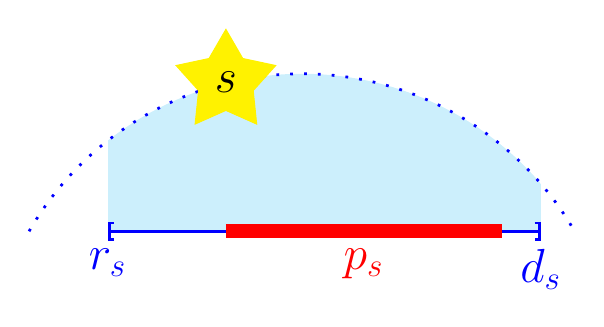
\begin{tikzpicture}
      \def\mypath{(0,0) arc[x radius=4cm, y radius=4cm, start angle=150, end angle=30]};
      
      \begin{scope}
        \clip\mypath;
        \fill[fill=cyan!20!] (1,0) rectangle (6.5,2.5);
      \end{scope}
      
      \draw[line width=1pt, color=blue, loosely dotted] \mypath;
      
      \node[star, star point height=3mm, minimum size=5mm, draw,
      color=yellow,fill=yellow,text=black] at (2.5,1.9) {\LARGE $s$};
      
      \draw[line width=1pt,color=blue,arrows={Bracket-Bracket}] (1,0)--(6.5,0);
      \node[below,blue] at (1,-.1) {\LARGE $r_s$};
      \node[below,blue] at (6.5,-.1) {\LARGE $d_s$};
      \draw[line width=5pt, color=red] (2.5,0) -- (6,0);
      \node[below,red] at (4.25,-.1) {\LARGE $p_s$};
    \end{tikzpicture}
  \end{minipage}
  \hfill
  \begin{minipage}{.3\linewidth}\footnotesize
    \begin{itemize}
    \item $[r_s;d_s)$ is the visibility interval 
    \item $p_s$ is the required duration of observation 
    \item $w_s$ is the interest 
    \end{itemize}
  \end{minipage}

  \vfill

  \begin{center}
  scheduling the observation of star $s$ means observing $s$ for a
  continuous duration $p_s$ within the visibility interval
  $[r_s;d_s)$, rewarding $w_s$
    
  \end{center}
  %%
  \note{%
    A star is only visible in the sky for a limited amount of time
    and, depending on the star position, the telescope possibilities,
    and the nature of the observation, one can compute a visibility
    interval during which the observation may occur.
    %
  }
\end{frame}

%% -----------------------------------------------------------------------------
\begin{frame}
  \frametitle{Star scheduling (one night)}

  Instance: a set \alert{$\cal S$} of stars; each star $s\in\cal S$
  has an interest \alert{$w_s$}, an observation duration \alert{$p_s$}
  and a visibility window \alert{$[r_s;d_s)$}
    
  \vfill

  \only<1>{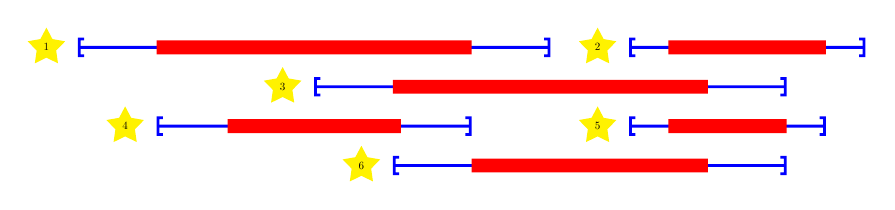
\begin{tikzpicture}
    % \mystar{y}{r}{d-r}{t-r}{p}{nom}
    \mystar{1.5}{0}{6}{1}{4}{$1$}{1}
    \mystar{1.5}{7}{3}{.5}{2}{$2$}{1}
    \mystar{1.0}{3}{6}{1}{4}{$3$}{1}
    \mystar{0.5}{1}{4}{0.9}{2.2}{$4$}{1}
    \mystar{0.5}{7}{2.5}{0.5}{1.5}{$5$}{1}
    \mystar{  0}{4}{5}{1}{3}{$6$}{1}
  \end{tikzpicture}}
  \only<2>{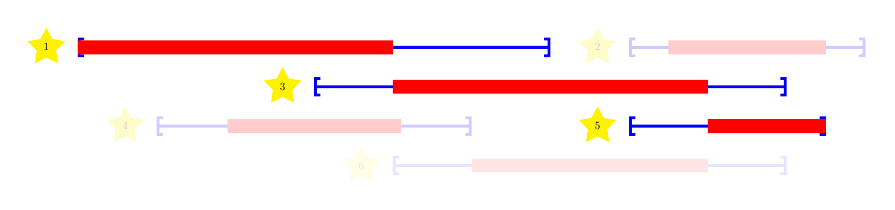
\begin{tikzpicture}
    % \mystar{y}{r}{d-r}{t-r}{p}{nom}
    \mystar{1.5}{0}{6}{    0}{4}{$1$}{1}
    \mystar{1.5}{7}{3}{   .5}{2}{$2$}{.2}
    \mystar{1.0}{3}{6}{    1}{4}{$3$}{1}
    \mystar{0.5}{1}{4}{  0.9}{2.2}{$4$}{.2}
    \mystar{0.5}{7}{2.5}{  1}{1.5}{$5$}{1}
    \mystar{  0}{4}{5}{    1}{3}{$6$}{.1}
  \end{tikzpicture}}


  \vfill

  \visible<2->{%
    Question: find $\cal \alert{S'} \subset S$ and starting times
    $\alert{t_s}, \forall s\in\cal S'$ such that
    \begin{itemize}
    \item for each $s\in\cal S'$: $[t_s; t_s+p_s) \subset [r_s;d_s)$
    \item for each $(s_1,s_2)\in{\cal S'}^2: [t_{s_1};
      t_{s_1}+p_{s_1})\cap[t_{s_2}; t_{s_2}+p_{s_2}) = \emptyset$
    \item $\sum_{s\in\cal S'} w_s$ is maximized
    \end{itemize}
  }
\end{frame}

%% -----------------------------------------------------------------------------
\begin{frame}
  \frametitle{Star scheduling (several nights)}

  Instance: a set \alert{$\cal N$} of nights, a set \alert{$\cal S$}
  of stars; each star $s\in\cal S$ has an interest \alert{$w_s$}, an
  observation duration \alert{$p_s^n$} and a visibility window
  \alert{$[r_s^n;d_s^n)$}, depending on the night $n$ of the
  observation
  
  \vfill
  
  \only<1>{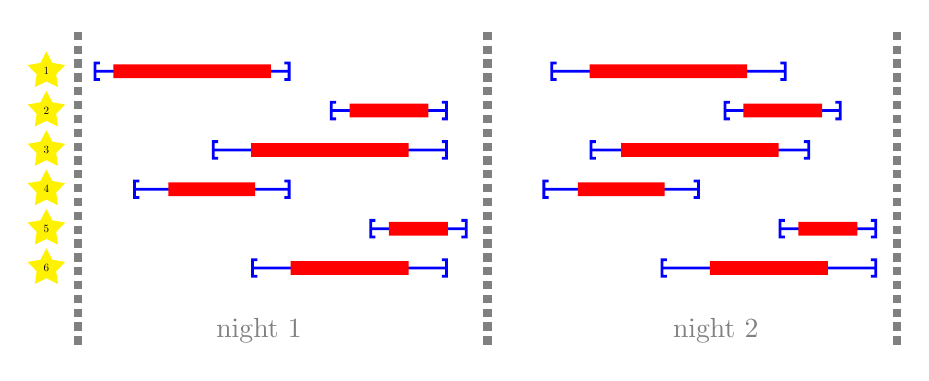
\begin{tikzpicture}
    % \mystar{y}{r}{d-r}{t-r}{p}{nom}
    \mystaronly{2.5}{-.2}{$1$}{1}
    \mystaronly{2.0}{-.2}{$2$}{1}
    \mystaronly{1.5}{-.2}{$3$}{1}
    \mystaronly{1.0}{-.2}{$4$}{1}
    \mystaronly{0.5}{-.2}{$5$}{1}
    \mystaronly{0.0}{-.2}{$6$}{1}
    \mystar{2.5}{  0}{2.5}{0.25}{2}{}{1}     \mystar{2.5}{5.8}{3.0}{0.5}{2}{}{1}
    \mystar{2.0}{3.0}{1.5}{.25}{1}{}{1}      \mystar{2.0}{8.0}{1.5}{.25}{1}{}{1}
    \mystar{1.5}{1.5}{3.0}{0.5}{2}{}{1}      \mystar{1.5}{6.3}{2.8}{0.4}{2}{}{1}
    \mystar{1.0}{0.5}{2.0}{0.45}{1.1}{}{1}   \mystar{1.0}{5.7}{2.0}{0.45}{1.1}{}{1}
    \mystar{0.5}{3.5}{1.25}{0.25}{0.75}{}{1} \mystar{0.5}{8.7}{1.25}{0.25}{0.75}{}{1}
    \mystar{  0}{  2}{ 2.5}{.5}{1.5}{}{1}    \mystar{  0}{7.2}{2.75}{.625}{1.5}{}{1}

    \draw[color=gray,dotted,line width=3pt] (.2,3)--(.2,-1) (5.4,3)--(5.4,-1) (10.6,3)--(10.6,-1);

    \node [gray] at (2.5,-.8) {night 1};
    \node [gray] at (8.3,-.8) {night 2};
  \end{tikzpicture}}%
  \only<2>{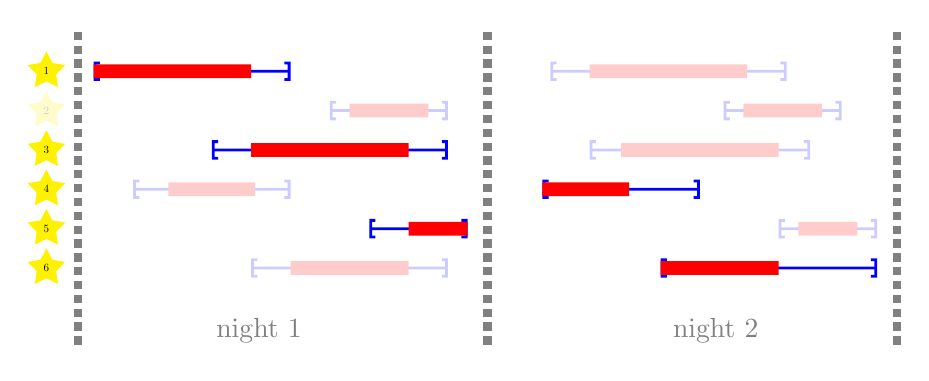
\begin{tikzpicture}
    % \mystar{y}{r}{d-r}{t-r}{p}{nom}
    \mystaronly{2.5}{-.2}{$1$}{1}
    \mystaronly{2.0}{-.2}{$2$}{.2}
    \mystaronly{1.5}{-.2}{$3$}{1}
    \mystaronly{1.0}{-.2}{$4$}{1}
    \mystaronly{0.5}{-.2}{$5$}{1}
    \mystaronly{0.0}{-.2}{$6$}{1}
    \mystar{2.5}{  0}{2.5}{0}{2}{}{1}        \mystar{2.5}{5.8}{3.0}{0.5}{2}{}{.2}
    \mystar{2.0}{3.0}{1.5}{.25}{1}{}{.2}     \mystar{2.0}{8.0}{1.5}{.25}{1}{}{.2}
    \mystar{1.5}{1.5}{3.0}{0.5}{2}{}{1}      \mystar{1.5}{6.3}{2.8}{0.4}{2}{}{.2}
    \mystar{1.0}{0.5}{2.0}{0.45}{1.1}{}{.2}  \mystar{1.0}{5.7}{2.0}{0   }{1.1}{}{1}
    \mystar{0.5}{3.5}{1.25}{0.5}{0.75}{}{1}  \mystar{0.5}{8.7}{1.25}{0.25}{0.75}{}{.2}
    \mystar{  0}{  2}{ 2.5}{.5}{1.5}{}{.2}   \mystar{  0}{7.2}{2.75}{0   }{1.5}{}{1}

    \draw[color=gray,dotted,line width=3pt] (.2,3)--(.2,-1) (5.4,3)--(5.4,-1) (10.6,3)--(10.6,-1);

    \node [gray] at (2.5,-.8) {night 1};
    \node [gray] at (8.3,-.8) {night 2};
  \end{tikzpicture}}
  

\end{frame}

%% -----------------------------------------------------------------------------
\begin{frame}
  \frametitle{The order is known!}
  
  The meridian instant ($m_s = \frac{r_s+d_s}{2}$) is a
  \alert{mandatory} instant of observation, that is: for every star
  $s$, \alert{$p_s^n \ge \frac{d_s^n-r_s^n}{2}$}

  \vfill

  \begin{center}%
    \only<1>{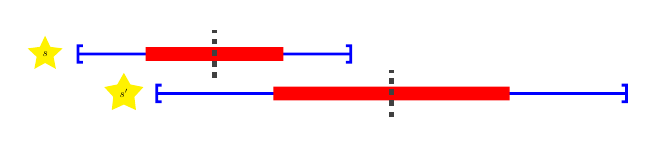
\begin{tikzpicture}
        \mystar{0.5}{0}{3.5}{0.875}{1.75}{$s$}{1}
        \mystar{0.0}{1}{6}{1.5}{3}{$s'$}{1}
        \draw[line width=2pt,dotted,darkgray]%
        (2.15, 0.2)--(2.15,0.8)
        (4.4,-0.3)--(4.4,0.3);
      \end{tikzpicture}}%
    \only<2>{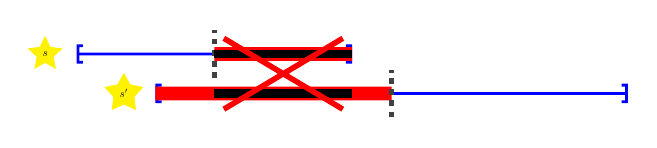
\begin{tikzpicture}
        \mystar{0.5}{0}{3.5}{1.75}{1.75}{$s$}{1}
        \mystar{0.0}{1}{6}{0}{3}{$s'$}{1}
        \draw[line width=2pt,dotted,darkgray]%
        (2.15, 0.2)--(2.15,0.8)
        (4.4,-0.3)--(4.4,0.3);
        \draw[line width=3pt,black] (2.15,0.5)--+(1.75,0) (2.15,0)--+(1.75,0);
        \draw[line width=2pt,red] (2.27,0.7)--(3.78,-0.2) (2.27,-0.2)--(3.78,0.7);
      \end{tikzpicture}}%
    \only<3>{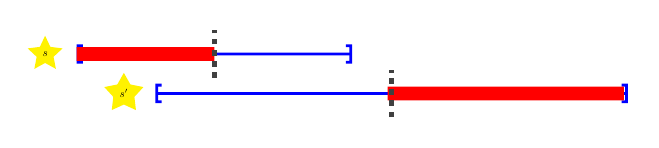
\begin{tikzpicture}
        \mystar{0.5}{0}{3.5}{0}{1.75}{$s$}{1}
        \mystar{0.0}{1}{6}{2.95}{3}{$s'$}{1}
        \draw[line width=2pt,dotted,darkgray]%
        (2.15, 0.2)--(2.15,0.8)
        (4.4,-0.3)--(4.4,0.3);
      \end{tikzpicture}}%
  \end{center}

  \vfill

  \begin{alertblock}{Property}
    If for all star $s$: $p_s^n \ge \frac{d_s^n-r_s^n}{2}$, then
    observations must be scheduled by non-decreasing meridian time
  \end{alertblock}
\end{frame}

%% -----------------------------------------------------------------------------
\begin{frame}
  \frametitle{A MIP model}
  \[
  \def\x{\vrule height 5mm depth 5mm width 0mm}
  \begin{array}{rl}
    \max & \displaystyle\sum_{s\in\cal S}w_s\,%
    \ghostput(-3.1mm,-3.8mm){
      \def\x{\vrule width 2mm height 2mm depth 0mm}
      \tikz{%
        \draw[color=red] (0,0) node[draw,fill=yellow,text=yellow](x) {\x};%
        \draw[->,color=red] (x) -- +(1.3,0) node[right] {$=1$ iff $s$ observed};%
      }
    } z_s \\
    s.c.
    \x & \displaystyle\sum_{n\in\cal N} %
    \ghostput(-3mm,-4mm){
      \def\x{\vrule width 2mm height 2mm depth 0mm}
      \tikz{%
        \draw[color=red] (0,0) node[draw,fill=yellow,text=yellow](x) {\x};%
        \draw[->,color=red] (x) ..controls +(0.5,0.3) .. +(1.8,0) node[right] {\hbox{$=1$ iff $s$ observed on night $n$}};%
      }
    }z_s^n = z_s \\
    \visible<2->{
      \ghostput(-35mm,-3mm){
        \color{green!30!black!70!}
        \begin{tabular}{r}visibility window\\of night $n$\end{tabular}
        $\left.\vrule height 7mm depth 7mm width 0mm\right\{$
      }
      %
      \x & r_s^nz_s^n \le %
      \ghostput(-3mm,-4mm){
        \def\x{\vrule width 2mm height 2mm depth 0mm}
        \tikz{%
          \draw[color=red] (0,0) node[draw,fill=yellow,text=yellow](x) {\x};%
          \draw[->,color=red] (x) -- +(1.3,0) node[right] {\hbox{starting time of observation $s$}};%
        }
      }t_s \\
      \x & t_s + p_s^nz_s^n \le d_s^nz_s^n + M(1-z_s^n) \\
    }
    \visible<3->{
      \ghostput(-37mm,-4mm){
        \color{green!30!black!70!}
        \begin{tabular}{r}$s \prec s'$ if observed\\the same night\end{tabular}
        $\left.\vrule height 7mm depth 7mm width 0mm\right\{$
      }
      %
      \x & z_s^n + z_{s'}^n -1 \le %
      \ghostput(-3mm,-4mm){
        \def\x{\vrule width 3.5mm height 2mm depth 0mm}
        \tikz{%
          \draw[color=red] (0,0) node[draw,fill=yellow,text=yellow](x) {\x};%
          \draw[->,color=red] (x) -- +(0.8,0) node[right] {\hbox{$=1$ iff $s$ and $s'$ observed}};
          \node[right,red] at +(2.3,-0.5) {the same night};%
        }
    }y_{ss'} \\
      \x & t_s + p_s^n \le t_{s'} + M(1-z_{ss'})
    }
  \end{array}\]
\end{frame}

%% -----------------------------------------------------------------------------
\begin{frame}[t]
  \vfill
  \tableofcontents[sectionstyle=show,subsectionstyle=show/show/show]%
\end{frame}


% ============================================================================
\section{Complexity}
\subsection{}%The one night case}

%% -----------------------------------------------------------------------------
\begin{frame}
  \frametitle{Scheduling one night}
  
  Instance: a set $\cal S$ of stars; each star $s\in\cal S$ has an
  interest $w_s$, an observation duration $p_s$ and a visibility
  window $[r_s;d_s)$ \alert{such that $p_s\ge (d_s-r_s)/2$}; a bound
  $W$

  Question: find a subset of stars so that the total interest is at
  least $W$, visibility windows are respected and observations do not
  overlap

  \vfill

  \begin{itemize}
  \item<2-> $1|r_j|\sum w_jU_j$ is NP-complete (Lenstra et al., 1977)
  \item<3-> $1|r_j,p_j=p|\sum w_jU_j$ is polynomial (Baptiste, 1999)
  \item<4-> what if $p_j\ge (d_j-r_j)/2$?
  \end{itemize}

  \vfill
  
  \visible<5>{\begin{alertblock}{Complexity of the one night case}
      Star scheduling of one night is NP-Hard (even if $w_s=1$)
  \end{alertblock}}

\end{frame}

%% -----------------------------------------------------------------------------
\begin{frame}
  \frametitle{Scheduling of one night is NP-hard}

  \begin{itemize}[<+->]
  \item Variant of Partition~: $2n$ pairs $(a_{2i-1},a_{2i})$ so that
    $\sum_i a_i=2B$. Can a total of $B$ be made with one item from
    each pair?% so that the total sum is $B$?

  \item For each pair of items $(a_{2i},a_{2i+1})$ create a pair of
    incompatible stars $(s_{2i-1},s_{2i})$: same visibility window and
    $p_s\ge(d_s-r_s)/2$

  \item Set visibility windows so that scheduling a star from a pair
    does not prevent scheduling a star from another pair and each pair
    of stars have dedicated
    instants%times when only those stars can be scheduled

  \item ``yes'' to Partition $\iff$ non-idling schedule of length
    $(2n+1)B$\kern-2mm
  \end{itemize}

  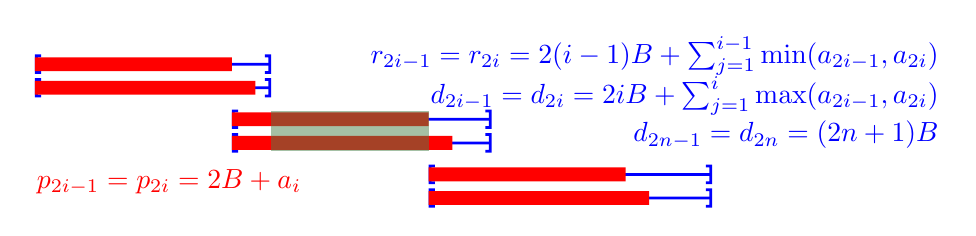
\begin{tikzpicture}
    \visible<2->{
      \mystar{1.7}{0}{3}{0}{2.5}{}{1}
      \mystar{1.4}{0}{3}{0}{2.8}{}{1}
    }
    \visible<3->{
      \mystar{1.0}{2.5}{3.3}{0}{2.5}{}{1}
      \mystar{0.7}{2.5}{3.3}{0}{2.8}{}{1}
      \mystar{0.3}{5.0}{3.6}{0}{2.5}{}{1}
      \mystar{0.0}{5.0}{3.6}{0}{2.8}{}{1}
      
      \fill[opacity=.5,green!30!black!70!] (3.4,1.1)--(3.4,0.6)--(5.4,0.6)--(5.4,1.1)--cycle;
    }
    
    \visible<2->{
      \node[red,right]  at (0.3,0.2) {$p_{2i-1}=p_{2i} = 2B + a_i$};
    }
    
    \visible<3->{
      \node[blue,left] at (12,1.8) {$r_{2i-1} = r_{2i} = 2(i-1)B + \sum_{j=1}^{i-1}\min(a_{2i-1},a_{2i})$};
      \node[blue,left] at (12,1.3) {$d_{2i-1} = d_{2i} = 2iB + \sum_{j=1}^i\max(a_{2i-1},a_{2i})$};

      \node[blue,left] at (12,0.8) {$d_{2n-1} = d_{2n} = (2n+1)B$};
    }
    
  \end{tikzpicture}%
  \note{%
    ***a schedule of cost *** is non-idling, thus at least a star
    among (2k-1;2k) has been chosen, which is a valid solution
    solution to Partition

    ***a solution to Partition is a schedule without idle time
    (because of costs) }
\end{frame}

%% -----------------------------------------------------------------------------
\begin{frame}
  \frametitle{A pseudo-polynomial algorithm}
  
  $f(i,t)$: maximum interest with stars 1 to $i$, and such that $s_i$
  ends before time $t$
  
  \vfill

  $f(i,t)=$\par\kern-5mm%
  \[\left\{
    \begin{array}{ll}
      \min( f(i-1,t), f(i-1,t - p_i) + w_i) & \forall i \in [1, m], t \in[r_i+p_i, T] \\
      f(i-1,t) & \forall i \in [1, m], t \in [0, r_i+p_i[ \\
      
      -\infty& \forall i \in [1, m], t < 0\\
      0	& i = 0, \forall t \in[0, T] 
    \end{array}
  \right.\]
  \vfill
  
  We are looking for $f(m,T)$ which can be computed in $O(mT)$
\end{frame}

%% TODO: can be extended to any fixed number of nights. Unique assumption: the order of the meridian is the same on each night (p_s^n mais differ, some stars may not be available, etc)

%% -----------------------------------------------------------------------------
\begin{frame}
  \frametitle{Scheduling several nights}
  
  Instance: a set of $n$ nights, a set $\cal S$ of stars; each star
  $s\in\cal S$ has an interest $w_s$, an observation duration $p_s^n$
  and a visibility window $[r_s^n;d_s^n)$ \alert{such that $p_s^n\ge
    (d_s^n-r_s^n)/2$}; a bound $W$

  Question: find a subset of stars so that the total interest is at
  least $W$, visibility windows are respected and observations do not
  overlap

  \vfill

  \begin{itemize}
  \item<2-> $P|r_j|\sum w_jU_j$ (identical nights) is NP-complete
  \item<3-> $p_s = (d_s-r_s)$, identical nights: polynomial (Kolen et al., 2007)
  \item<4-> what if $p_j\ge (d_j-r_j)/2$?
  \end{itemize}

  \vfill
  
  \visible<5>{\begin{alertblock}{Complexity of the several nights
        case} Star scheduling of several nights is unary NP-Hard (even
      if $w_s=1$ and all nights are identical)
  \end{alertblock}}
  % 
  \note{%
    Reduction from Numerical 3-Dimensional Matching
  }
\end{frame}

% ============================================================================
\section[Solutions]{Solving star scheduling}
\subsection{}%Solution methods}

%% -----------------------------------------------------------------------------
\begin{frame}
  \frametitle{Logic-based Bender decomposition}
  \begin{columns}[t]
    \begin{column}{.5\textwidth}
      Master problem: \\
      assignment of stars to nights

      \[\begin{array}{rl}
        \max & \displaystyle\sum_{s\in\cal S}w_s z_s \\
        s.c. & \displaystyle\sum_{n\in\cal N} z_s^n = z_s 
        \ghostput(5mm,-8mm){\visible<2->{\tikz{\draw[->] (0,0) -- (1.9,.7); \draw[->] (0,0) -- (1.9,-.2);}}}
        \\
        &\visible<3->{\alert{\displaystyle\sum_{s\in C_k^n} z_s^n \le |C_k^n| - 1%
          \ghostput(1.55mm,-16.5mm){\visible<2->{\tikz{\draw[->,red] (1,1.5) -- (0,0.1); \draw[->,red] (1,0.6) -- (0,0);}}}}

        }
      \end{array}\]

      \begin{itemize}[<4->]
      \item efficient MIP
      \item upper bound at each iteration
      \end{itemize}
    \end{column}
    % 
    \begin{column}{.5\textwidth}
      \visible<2->{%
      Slave problem: \\
      scheduling of each nights 

      \kern1cm

      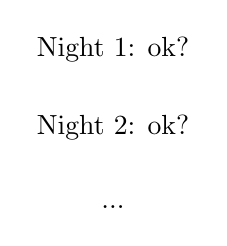
\begin{tikzpicture}
        \node[rectangle] at (0,2) {Night 1: ok?};
        \node[rectangle] at (0,1) {Night 2: ok?};
        \node[rectangle] at (0,0) {...};
      \end{tikzpicture}
      }
      
      \kern6mm
  
      \begin{itemize}[<4->]
      \item $n$ independent problems
      \item linear complexity
      \end{itemize}
    \end{column}
  \end{columns}
\end{frame}

%% -----------------------------------------------------------------------------
\begin{frame}
  \frametitle{Column generation}
  
  Night patterns: \alert{$\Omega_n$}, set of all possible schedules
  for night $n$

  Pattern $k$ for night $n$: $p_{n1}^k...p_{n|\cal S|}^k$, where
  $\alert{p_{ns}^k}=1$ iff star $s$ belongs to the $k$-th pattern of
  night $n$; weight $\alert{w_n^k} = \sum_{s\in\cal S}w_sp_{ns}^k$

  \visible<2->{
  \[\begin{array}{lrcll}
    & \max \sum_{n\in\cal N}\sum_{k \in {\Omega_n}} w^{k}_n%
        \ghostput(-3mm,-3.9mm){
      \def\x{\vrule width 2mm height 2.5mm depth 0mm}
      \tikz{%
        \draw[color=alert] (0,0) node[draw,fill=yellow,text=yellow](x) {\x};%
        \draw[->,color=alert] (x) -- +(1.1,0) node[right] {$=1$ iff pattern $k$ used, night $n$};%
      }
    } \rho^{k}_{n}%
    & & & \\
    \visible<3->{\color{green!30!black!70!}\alpha_n}
   & \sum_{k \in \Omega_n}\rho^{k}_{n}  &=& 1 & \forall n \in {\cal N} \\
    \visible<3->{\color{green!30!black!70!}\beta_s}
   & \sum_{n\in\cal N}\sum_{k \in \Omega_n} p^{k}_{ns}\rho^{k}_{n} &\leq& 1& \forall s \in {\cal S}\\
  &  \rho^k_n \in \{0,1\} && & \forall n \in {\cal N}, \forall k \in {\Omega_n}
 \end{array}\]
 }
 
 \vfill 

 \visible<3->{Reduced cost of $\rho_n^k$: $w_n^k - \alpha_n -
   \sum_{s\in\cal S}p_{ns}^k\beta_s
   % = - \alpha_n + \sum_{s\in\cal S}(w_s-\beta_s)p_{ns}^k
   $

}

 \vfill 

 \visible<4->{Pattern of max reduced cost? Single Night Case with
   costs $w_s-\beta_s$ }
\end{frame}

%% -----------------------------------------------------------------------------
\begin{frame}
  \frametitle{Local search}

  Classical local-search procedure

  \vfill

  Neighborhoods:
  \begin{itemize}
  \item moving a star from one night to another
  \item inserting an unobserved star
  \item exchanging two stars
  \end{itemize}
  An optimal schedule for each night is computed systematically
\end{frame}

% %% -----------------------------------------------------------------------------
% \subsection{Experimental results}

%% -----------------------------------------------------------------------------
\begin{frame}
  \frametitle{Solutions}

  {\small\def\x{\bfseries}\def\y{\itshape}
    \leavevmode\kern-3mm
  \begin{tabular}{|l|rr|rr|rr|rr|}
    \hline
    &&    
    & \multicolumn{2}{|c|}{BD (OPT/\textit{UB})} 
    & \multicolumn{2}{|c|}{CG (UB)} 
    & \multicolumn{2}{|c|}{LS (LB)} 
    \\
    instance & $|\cal S|$ & $|\cal N|$ 
    & val & cpu(s)
    & val & cpu(s)
    & val & cpu(s)
    \\
    \hline
    pb1  & 200 &  32 &\y\x 5200 & 900 & \x 5200 &  1.47 & \x 5200 & 0.28 \\
    pb2  & 200 &  32 &\y\x 3310 & 900 & \x 3310 &  0.99 & \x 3310 & 0.33 \\
    pb3  & 200 &  69 &  \x 7800 & 100 & \x 7800 &  1.59 & \x 7800 & 0.17 \\
    pb4  & 200 &  69 &   -      &  -  & \x 4870 &  1.63 & \x 4870 & 0.11 \\
    pb5  & 400 &  69 &\y  12660 & 900 &\x 11910 &  5.11 &\x 11910 &12.39 \\
    pb6  & 400 &  69 &\y   9250 & 900 &  9099.9 & 19.57 &    9070 &773.95\\
    pb7  & 400 & 142 &   -      &  -  &\x 13680 & 11.85 &\x 13680 & 0.15 \\
    pb8  & 400 & 142 &\y\x 9760 & 900 & \x 9760 & 13.71 & \x 9760 & 0.21 \\
    \hline
    real & 800 & 142 &\y  18930 & 900 &   18620 & 92.41 &   18510 &689.60\\
         &     &     &          &     &         &       &   18480 &306.07\\
    \hline
  \end{tabular}}
%  pb6 gap 0.22 \\
%  reeal ap 0.16 \\
\end{frame}
%%***TODO: pb4 : erreur dans le tableau de résultats ? Benders donne solution non opt alors qu'il s'arrête en 150s avec moins que l'OPT !!!

%% -----------------------------------------------------------------------------
\begin{frame}
  \frametitle{Example solution}
  \pgfimage[width=\textwidth]{solution}
\end{frame}


% ============================================================================
\section[Conclusions]{Conclusions and perspectives}
\subsection{}

%% -----------------------------------------------------------------------------
\begin{frame}
  \frametitle{Star scheduling}
  \begin{itemize}
  \item a particular interval-scheduling problem with known order
  \item NP-hardness is proven for both one night and general cases
  \item several solution methods are proposed and tested
  \end{itemize}
\end{frame}

%% -----------------------------------------------------------------------------
\begin{frame}
  \frametitle{Work in progress...}
  \begin{itemize}

  \item Instances
    \begin{itemize}
    \item we need more instances!
    \item study the structure of the real instance \\ (e.g.,
      similarity between nights)
    \end{itemize}

    \vfill

  \item Solution methods
    \begin{itemize}
    \item enrich numerical experiments
    \item embed the CG into a branch \& bound to get optimal solutions
    \item analyze (and improve) LS behavior
    \item get advantage of nights' similarities
    \end{itemize}

    \vfill

  \item Complexity
    \begin{itemize}
    \item draw precise complexity frontiers
    \item study approximability
    \end{itemize}
  \end{itemize}

\end{frame}


\end{document}
